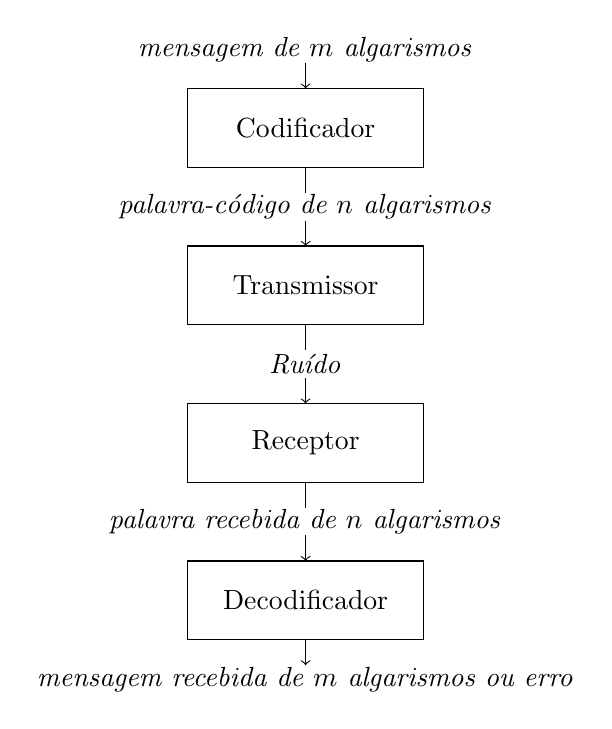
\begin{tikzpicture}[scale=1]

\coordinate (m-digit-message) at (0,8);
\coordinate (encoder) at (0,7);
\coordinate (n-digit-code-word) at (0,6);
\coordinate (transmitter) at (0,5);
\coordinate (noise) at (0,4);
\coordinate (receiver) at (0,3);
\coordinate (n-digit-received-word) at (0,2);
\coordinate (decoder) at (0,1);
\coordinate (m-digit-received-message) at (0,0);

\coordinate (encoder-rectangle-left) at (-1.5,6.5);
\coordinate (encoder-rectangle-right) at (1.5,7.5);
\coordinate (encoder-rectangle-top) at (0,7.5);
\coordinate (encoder-rectangle-bottom) at (0,6.5);

\coordinate (transmitter-rectangle-left) at (-1.5,4.5);
\coordinate (transmitter-rectangle-right) at (1.5,5.5);
\coordinate (transmitter-rectangle-top) at (0,5.5);
\coordinate (transmitter-rectangle-bottom) at (0,4.5);

\coordinate (receiver-rectangle-left) at (-1.5,2.5);
\coordinate (receiver-rectangle-right) at (1.5,3.5);
\coordinate (receiver-rectangle-top) at (0,3.5);
\coordinate (receiver-rectangle-bottom) at (0,2.5);

\coordinate (decoder-rectangle-left) at (-1.5,0.5);
\coordinate (decoder-rectangle-right) at (1.5,1.5);
\coordinate (decoder-rectangle-top) at (0,1.5);
\coordinate (decoder-rectangle-bottom) at (0,0.5);

\draw [->] ([yshift=-5]m-digit-message) -- (encoder-rectangle-top); 
\draw (encoder-rectangle-left) rectangle  (encoder-rectangle-right);
\draw (encoder-rectangle-bottom) -- ([yshift=5]n-digit-code-word);

\draw [->] ([yshift=-5]n-digit-code-word) -- (transmitter-rectangle-top); 
\draw (transmitter-rectangle-left) rectangle  (transmitter-rectangle-right);
\draw (transmitter-rectangle-bottom) -- ([yshift=5]noise);

\draw [->] ([yshift=-5]noise) -- (receiver-rectangle-top); 
\draw (receiver-rectangle-left) rectangle  (receiver-rectangle-right);
\draw (receiver-rectangle-bottom) -- ([yshift=5]n-digit-received-word);

\draw [->] ([yshift=-5]n-digit-received-word) -- (decoder-rectangle-top); 
\draw (decoder-rectangle-left) rectangle  (decoder-rectangle-right);
\draw [->] (decoder-rectangle-bottom) -- ([yshift=5]m-digit-received-message);

\node at (m-digit-message) {\emph{mensagem de $m$ algarismos}};
\node at (encoder) {Codificador};
\node at (n-digit-code-word) {\emph{palavra-código de $n$ algarismos}};
\node at (transmitter) {Transmissor};
\node at (noise) {\emph{Ruído}};
\node at (receiver) {Receptor};
\node at (n-digit-received-word) {\emph{palavra recebida de $n$ algarismos}};
\node at (decoder) {Decodificador};
\node at (m-digit-received-message) {\emph{mensagem recebida de $m$ algarismos ou erro}};

\end{tikzpicture}
